\section{Measurement quality}
\label{results:overview-and-measurement-quality}

Three measurement-quality checks precede the results for each research question. Section~\ref{results:overview-and-measurement-quality:run-completeness-and-result-agreement} establishes which configuration, workload, and tier cells completed and whether the configurations that ran a given workload returned matching result counts. Section~\ref{results:overview-and-measurement-quality:timing-distributions-and-estimator-behavior} describes how the per-iteration timings are distributed and why the minimum is the reported location estimator. Achieved iteration counts and the convergence of the sequential stopping rule are reported in Section~\ref{results:overview-and-measurement-quality:iteration-counts-and-convergence}.

\subsection{Run completeness and result agreement}
\label{results:overview-and-measurement-quality:run-completeness-and-result-agreement}

Figures~\ref{fig:results-coverage-single-machine} and~\ref{fig:results-coverage-distributed} record the completion status of every configuration, workload, and tier cell. On a single node, DuckDB over GeoParquet and PostGIS completed all three query patterns at both the small and large tiers, and GeoPandas over Shapefile completed all three at the small tier. The Shapefile cells beyond the small tier did not run by design. For the national-scale spatial join, the single-node DuckDB and PostGIS engines completed the small and medium tiers but did not complete the large tier, while the Apache Sedona broadcast strategy completed every tier at all worker counts. The partitioned strategy completed the small tier only. Its medium- and large-tier runs did not complete, recording an executor out-of-memory failure at every worker count. Where the twelve-worker runs completed, each cell holds \num{6} iterations rather than the \num{9} collected elsewhere: a defect in the benchmark code, corrected partway through execution, cost three iterations at that worker count, and rerunning the configuration to recover them was judged too costly.

Where more than one configuration ran the same workload, the returned result counts agreed closely; Table~\ref{tab:appendix-cardinality-agreement} reports the per-cell counts. The k-nearest-neighbor search, the point-in-polygon lookup, and the national-scale join returned identical counts across the engines that ran them, a maximum relative discrepancy of \num{0}\% in each case (\num{10}, one, and \num{357} rows respectively). The bounding-box filter was the only workload whose returned set differed measurably between engines, with DuckDB returning slightly more rows than PostGIS at both tiers and a maximum relative discrepancy of \num{1.53}\%.

\begin{figure}[H]
    \centering
    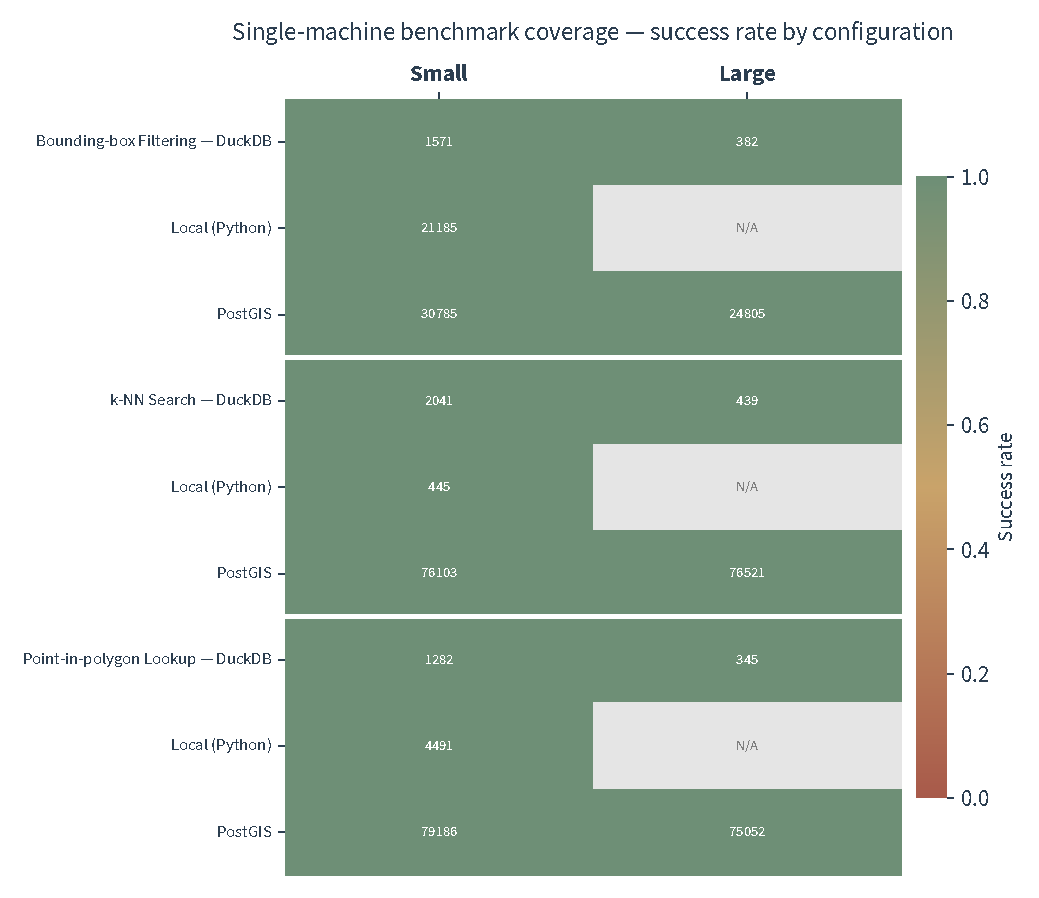
\includegraphics[width=0.85\textwidth]{Chapters/06-results/sub-chapters/figures/06-results-coverage-single-machine.pdf}
    \caption[Run-completeness coverage grid (single-machine)]{Completion status of
    every single-machine configuration across the three query patterns and the small
    and large tiers. Each cell records whether the run completed in full, completed
    partially under the sequential stopping rule, or did not run for that
    combination. Every Shapefile cell beyond the small tier is absent by design and
    is marked as did-not-run rather than as missing or failed cells.}
    \label{fig:results-coverage-single-machine}
\end{figure}

\begin{figure}[H]
    \centering
    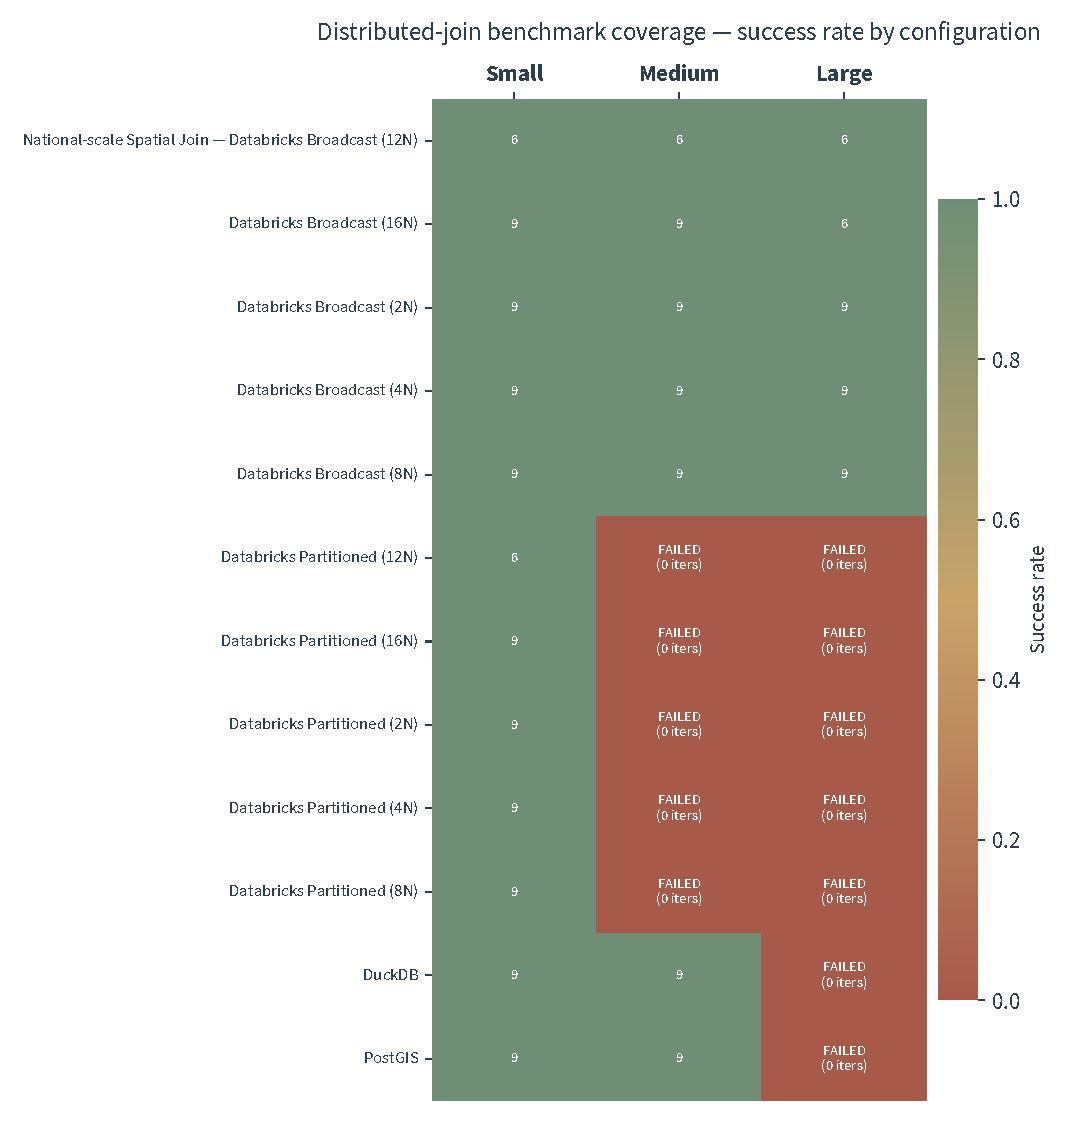
\includegraphics[width=0.85\textwidth]{Chapters/06-results/sub-chapters/figures/06-results-coverage-distributed.pdf}
    \caption[Run-completeness coverage grid (distributed join)]{Completion status of
    every configuration for the national-scale spatial join -- the single-node DuckDB
    and PostGIS engines and the Apache Sedona broadcast and partitioned variants at
    each worker count -- across the small, medium, and large tiers. Each cell records
    whether the run completed in full, completed partially, or failed or did not run
    for that combination.}
    \label{fig:results-coverage-distributed}
\end{figure}

\subsection{Timing distributions and estimator behavior}
\label{results:overview-and-measurement-quality:timing-distributions-and-estimator-behavior}

Figure~\ref{fig:results-warmup} shows the per-iteration timing behavior for a representative cell, the point-in-polygon lookup on DuckDB over GeoParquet at the small tier. The distribution in panel~(a) rises off a hard lower bound and trails a long right tail, so the mean and the median both sit above the fastest observed iteration. This one-sided, right-skewed contamination is the shape the minimum estimator is chosen to reject (Section~\ref{research-design-and-methodology:statistical-analysis:summary-statistics-and-the-choice-of-estimator}). Figure~\ref{fig:appendix-estimator-illustration} reports the quantified separation between the minimum, the median, and the mean for this same cell. Panel~(b) plots elapsed time against iteration index within a single measurement pass. The per-iteration times scatter within a narrow band above the steady-state minimum, without a pronounced warmup ramp.

\begin{figure}[H]
    \centering
    \subfloat[Per-iteration elapsed-time distribution.\label{fig:results-warmup-distribution}]{%
        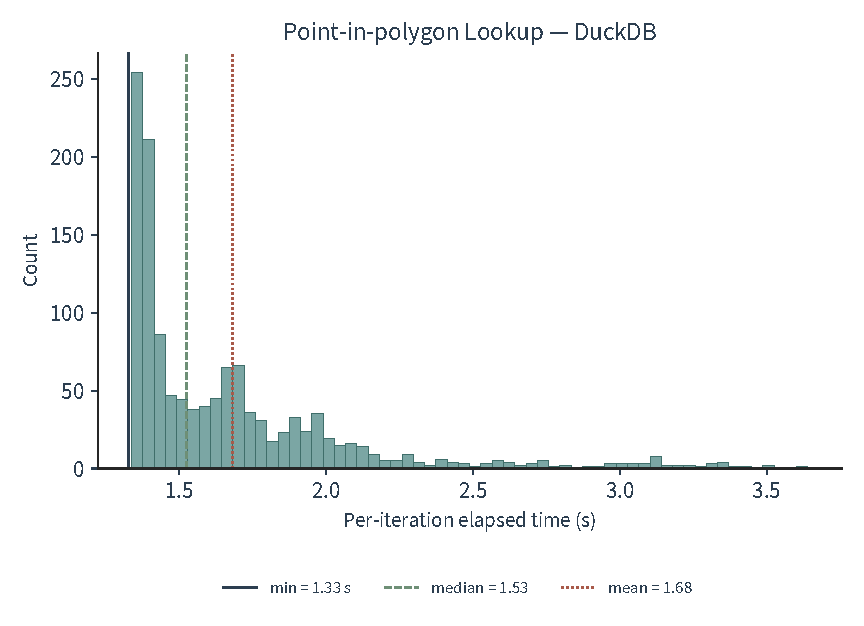
\includegraphics[valign=t, width=0.45\textwidth]{Chapters/06-results/sub-chapters/figures/06-results-warmup-distribution.pdf}}%
    \hfill
    \subfloat[Warmup-to-steady-state decay.\label{fig:results-warmup-decay}]{%
        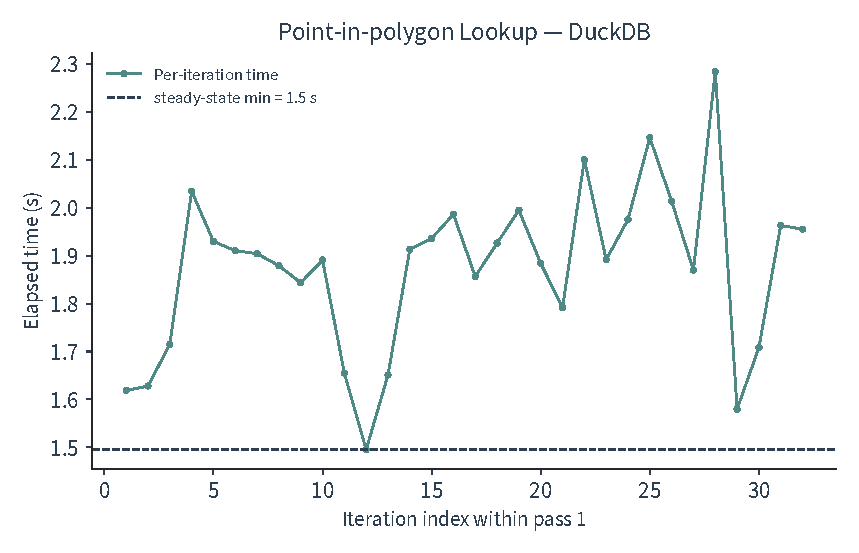
\includegraphics[valign=t, width=0.45\textwidth]{Chapters/06-results/sub-chapters/figures/06-results-warmup-decay.pdf}}%
    \caption[Per-iteration timing distribution and warmup behavior]{Per-iteration
    timing behavior for one representative configuration, workload, and tier (DuckDB
    over GeoParquet, point-in-polygon, small tier). Panel~(a) shows the distribution
    of per-iteration elapsed times, with its hard lower bound and the one-sided,
    right-skewed contamination that motivates reporting the minimum rather than the
    mean \parencite{chen2016_robust_benchmarking_noisy_environments}. Panel~(b) shows
    per-iteration elapsed time against iteration index within one measurement pass,
    fluctuating within a narrow band above the steady-state minimum (dashed).}
    \label{fig:results-warmup}
\end{figure}

\subsection{Iteration counts and convergence}
\label{results:overview-and-measurement-quality:iteration-counts-and-convergence}

Figure~\ref{fig:results-convergence} traces the sequential stopping rule for the same representative cell over a single measurement pass. The running half-width of the bootstrap confidence interval, expressed as a fraction of the running minimum, reaches the \num{5}\% relative target within the first iterations and stays close to it thereafter.

Table~\ref{tab:results-achieved-n} reports, for each single-machine cell, the achieved count of successful iterations, the minimum-estimator elapsed time, the final confidence-interval half-width, and the recorded stop reason. Every cell that ran reached the precision target rather than a budget or timeout limit. The achieved counts ranged across cells from \num{345} iterations for the point-in-polygon lookup on DuckDB at the large tier to \num{79186} for the same pattern on PostGIS at the small tier. The national-scale join took the fixed-iteration branch of the protocol rather than the sequential rule (Section~\ref{research-design-and-methodology:workloads:iteration-counts}), so its per-cell counts are reported with the distributed results in Table~\ref{tab:distributed-join-descriptive-statistics}.

\begin{figure}[H]
    \centering
    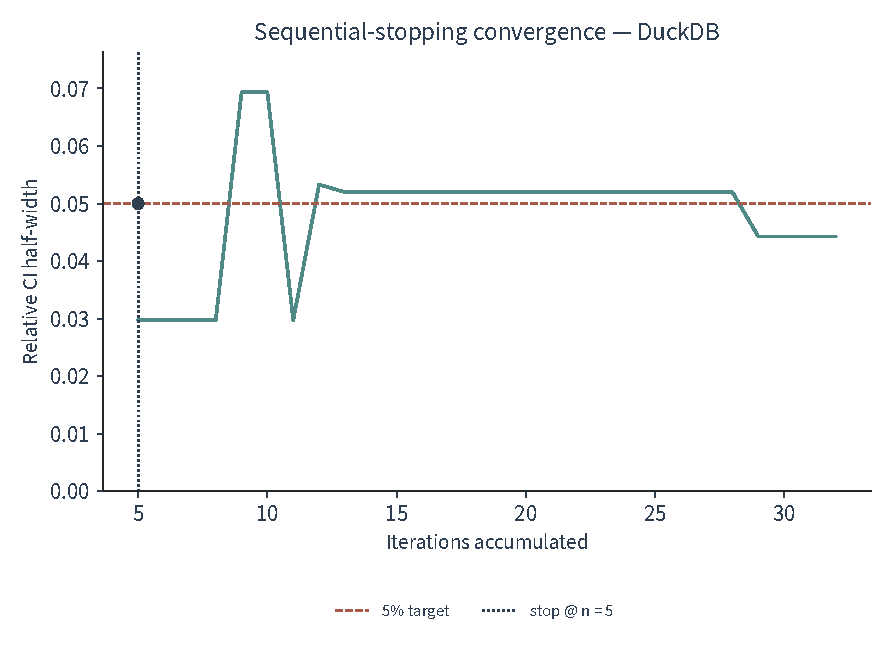
\includegraphics[width=0.7\textwidth]{Chapters/06-results/sub-chapters/figures/06-results-convergence.pdf}
    \caption[Sequential-stopping convergence]{Convergence of the sequential stopping
    rule for one representative configuration, workload, and tier (DuckDB over
    GeoParquet, point-in-polygon, small tier), over a single measurement pass. The
    running bootstrap \num{95}\% confidence-interval half-width, expressed as a
    fraction of the running minimum elapsed time, is plotted against the number of
    accumulated iterations; the horizontal line marks the \num{5}\% relative target
    half-width \parencite{georges2007_statistically_rigorous_java_performance,laaber2019_software_microbenchmarking_cloud},
    and the marker indicates the first iteration at which the running half-width meets
    that target.}
    \label{fig:results-convergence}
\end{figure}

\begin{table}[H]
    \centering
    \footnotesize
    \setlength{\tabcolsep}{6pt}
    \renewcommand{\arraystretch}{1.2}
    \resizebox{\textwidth}{!}{%
    \begin{tabular}{@{}l l l r r r l@{}}
        \toprule
        \textbf{Configuration} & \textbf{Workload} & \textbf{Tier} & \textbf{Achieved $n$} & \textbf{Min.\ (\si{\second})} & \textbf{\acrshort{ci} half-width} & \textbf{Stop reason} \\
        \midrule
        \inputtablebody{Chapters/06-results/sub-chapters/tables/06-achieved-iterations.tex}
        \bottomrule
    \end{tabular}}
    \caption[Achieved iteration counts and convergence]{Achieved count of successful
    timed iterations, minimum-estimator elapsed time, final bootstrap \num{95}\%
    confidence-interval half-width, and recorded stop reason for each single-machine
    configuration, query pattern, and size tier. The reported $n$ is the achieved
    number of successful iterations recorded in the run metadata, not the configured
    ceiling. Cells that did not run by design carry an explicit did-not-run stop
    reason rather than a zero count.}
    \label{tab:results-achieved-n}
\end{table}